\documentclass[a4paper, 11pt]{article}
\usepackage[utf8]{inputenc}
\usepackage{physics}
\usepackage{float}
\usepackage{graphicx}
\usepackage{amsmath}

\author{Kandidatnummer: 15010}
\title{FYS3410 - module I}

\begin{document}
\maketitle
	\section*{2: Hexagonal crystal structure}
		\begin{figure}[H]
			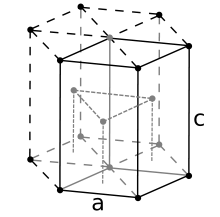
\includegraphics{hcp.png}
		\end{figure}
		\subsection*{a) number of atoms in the cell}
			There are four lattice points that are shared between six unit cells, four that are shared between twelve and one atom in the middle of the unit cell
			$$\frac{4}{6}+\frac{4}{12}+1 = 2$$
		\subsection*{b) calculating the characteristic c/a ratio}
			
\end{document}